The structure of the proposed control strategy is presented in \cref{fig:tikzControlStrat} and includes the aforementioned inner fast loop and outer slow loop:  

\begin{figure}[h!]
	\centering
	\resizebox{\columnwidth}{!}{
		\begin{tikzpicture}[auto, node distance=2.5cm,>=latex']
	% ========================== Nodes ============================
	% Nodes in upper vertical line
	\node [input, name=rinput] (rinput) {};
	\node [sum, right of=rinput] (sum1) {};
	\node [block, right of=sum1, node distance = 1.5cm] (LQR) {LQR};
	\node [sum, right of=LQR, node distance =
	1.5cm] (sum2) {};
	\node [block, right of=sum2, node distance = 1.5cm] (PID){PID};
	\node [block, right of=PID, align=center] (Fast){Fast\\Dynamics};
	\node [block, right of=Fast, node distance = 3cm, align=center] (Slow){Slow\\Dynamics};
	\node [output, right of=Slow] (output) {};
	
	% Nodes for inner feedback
	\node [tmp, right of=Fast, node distance = 1.5cm] (tmp0){};
	\node [tmp, below of=tmp0, node distance = 1.5cm] (tmp1){};
	\node [tmp, below of=sum2, node distance = 1.5cm] (tmp2){};
	
	% Nodes for outer feedback
	\node [tmp, right of=Slow, node distance = 1.5cm] (tmp10){};
	\node [tmp, below of=tmp10,node distance = 2.5cm] (tmp11){};
	\node [tmp, below of=sum1, node distance = 2.5cm] (tmp12){};
	
	% Nodes for Disturbance
	\node [tmp, above of=tmp0, node distance = 2.5cm] (tmp20){};
	\node [tmp, above of=tmp0, node distance = 2cm] (tmp21){};
	\node [tmp, above of=Fast, node distance = 2cm] (tmp22){};
	\node [tmp, above of=Slow, node distance = 2cm] (tmp23){};
	
	\draw[thick, dotted] ($(Fast.north west)+(-0.25, 0.25)$) rectangle  ($(Slow.south east)+(0.25, -0.25)$);
	\node[above of =tmp0, node distance =1.1cm](sys_txt) {System};
	
	% ========================== Lines ============================
	
	% Lines in upper vertical part of block diagram
	\draw [->] (rinput) -- node{$p_{ref}$} (sum1);
	\draw [->] (sum1) --node[name=z,anchor=north]{} (LQR);
	\draw [->] (LQR) -- node{$ q_{ref} $}(sum2);
	\draw [->] (sum2) -- (PID);
	\draw [->] (PID) -- node[pos=0.4]{$ \omega_{ref} $}(Fast);
	\draw [->] (Fast) -- node{$d_p$}(Slow);
	\draw [->] (Slow) -- node{$p_{\tau}$}(output);	
	
	% Lines for inner feedback
	\draw [-] (tmp0) -- (tmp1);
	\draw [-] (tmp1) -- (tmp2);
	\draw [->] (tmp2) -- node[pos=0.99]{$ - $}(sum2);
	
	
	% Lines for outer feedback
	\draw [-] (tmp10) -- (tmp11);
	\draw [-] (tmp11) -- (tmp12);
	\draw [->] (tmp12) -- node[pos=0.99]{$ - $}(sum1);
	
	
	% Lines for disturbance
	\draw [-] (tmp20)node[above, align=center]{Consumer \\ Disturbance} -- (tmp21);
	\draw [-] (tmp21) -- (tmp22);
	\draw [-] (tmp21) -- (tmp23);
	\draw [->] (tmp22) -- node[left, pos = 0.5]{$\Theta$}(Fast);
	\draw [->] (tmp23) -- node[pos = 0.5]{$ d_c $}(Slow);
	
	
\end{tikzpicture}
}
	\caption{Control Strategy including control for fast and slow dynamics}
	\label{fig:tikzControlStrat}
\end{figure}

\subsection{Outer Loop}\label{subsec:OuterLoop}

We will first address the outer LQR controller. This is an optimal controller that, in its continuous, LTI, infinite-horizon form, is given by the solution to the Lagrange problem:

\begin{equation}\label{eq:LagrangeProblem}
		J = \int_{t_0}^{\infty} \big(x^T(t)Qx(t) + u^T(t)Ru(t)\big)dt
\end{equation} 

constrained by the dynamics:

\begin{equation}\label{eq:LQRDynamicsConstraint}
	\begin{gathered}
		\dot{x}(t) = Ax(t) + Bu(t) \\
		x(t_0) = x_0
	\end{gathered} 
\end{equation}

The optimal solution to this problem is given by minimising the Hamiltonian $\mathcal{H}$ \cite{Liberzon2012}:

\begin{equation}\label{eq:Hamiltonian}
	\begin{gathered}
			\mathcal{H} = \lambda^T(t) f(x(t),u(t)) - \mathcal{L}(x(t),u(t)) \\
			f(x(t),u(t)) = A(t)x(t) + B(t)u(t) \\
			\mathcal{L}(x(t),u(t)) =  x^T(t)Q(t)x(t) - u^T(t)R(t)u(t)
	\end{gathered}
\end{equation}

which gives a solution of the type:

\begin{equation}\label{eq:LQRSolution}
	u^*(t) = -RB^TPx^*(t) = -Kx^*(t)
\end{equation}

where $P$ is the solution to the algebraic Riccatti equation:

\begin{equation}\label{eq:ARE}
	PA + A^TP + Q - PBR^{-1}B^TP = 0
\end{equation}

However, the standard LQR has several major issues. It only regulates to the origin, it does not have integral action, and it does not reject state disturbances. We therefore, as in Pannocchia et al. \cite{Pannocchia2015a}, rewrite the above as a discrete problem in deviation variables and solve:

\begin{equation}\label{eq:LagrangeProblemDeviation}
	\begin{gathered}
	J = \sum_{k_0}^{\infty} \big(\zeta(k)^TQ\zeta(k) + \tilde{u}(k)^TR\tilde{u}(k)\big) \\
	\zeta = \begin{bmatrix}	x(k)-x(k-1) \\ y(k)-r(k) \end{bmatrix}, \quad \tilde{u}(k) = u(k)-u(k-1) 
	\end{gathered}
\end{equation} 

where the constraining dynamics are given by:

\begin{equation}\label{eq:VelocityMatrices}
	\begin{gathered}
		\zeta(k+1) = \tilde{A}\zeta(k) + \tilde{B}\tilde{u}(k) \\
		\tilde{A} = \begin{bmatrix} A & 0 \\ CA & I	\end{bmatrix}, \ 
		\tilde{B} = \begin{bmatrix} B \\ CB	\end{bmatrix}, \ \tilde{C} = \begin{bmatrix} 0 & I	\end{bmatrix}
	\end{gathered}
\end{equation}

and the optimal control policy becomes:

\begin{equation}\label{eq:OptimalVFLQRPolicy}
\begin{gathered}
\tilde{u}^*(k)  = -\tilde{K}\tilde{x}^*(k) \\
\tilde{K} = (\tilde{B}^TP\tilde{B}-R)^{-1}(\tilde{B}^TP\tilde{A}) \\
u^*(k) = \sum_{i=1}^{k} \tilde{u}^*(i)
\end{gathered}
\end{equation}

where $P$ is now the solution to the \textit{discrete} algebraic Riccatti equation:

\begin{equation}\label{eq:DARE}
	-Q = \tilde{A}^TP\tilde{A} - P - (\tilde{A}^TP\tilde{B})(\tilde{B}^TP\tilde{B}+R)^{-1}(\tilde{B}^TP\tilde{A})
\end{equation}

This control policy clearly has tracking as $\zeta(k+1) = 0$ implies $y(k+1)-r(k+1) = 0$, and has integral action by virtue of its incremental form. However, it still lacks disturbance rejection. Assuming that we are only concerned with optimal control of the disturbance-free subsystem, complete rejection of the state disturbance $\delta(k)$ can then be achieved by augmenting \cref{eq:OptimalVFLQRPolicy} \cite{Singh2017}:

\begin{equation}
	u(k) = \sum_{i=1}^{k} \tilde{u}^*(k) - B^\dagger \mathcal{B}\delta(k)
\end{equation}

where $B^\dagger$ is the Moore-Penrose pseudoinverse of $B$ and $\mathcal{B}$ is the disturbance input matrix.

\subsection{Inner Loop}\label{subsec:InnerLoop}

We now address the inner loop and its PID controllers. The model used for their design is the state-space model of the fast dynamics given in \cref{eq:LinearisedModelWithTank}, with a Padé approximation of a $4$-second output delay included. This state-space system with output delay can be converted into the frequency-domain transfer matrix $G(s)$:

\begin{equation}\label{eq:TransferMatrix}
	G(s) = \begin{bmatrix} G_{11}(s) & G_{12}(s) \\ G_{21}(s) & G_{22}(s)\end{bmatrix}
\end{equation}

which can be shown to be approximately diagonal:

\begin{figure}[h!]
 	\centering
 	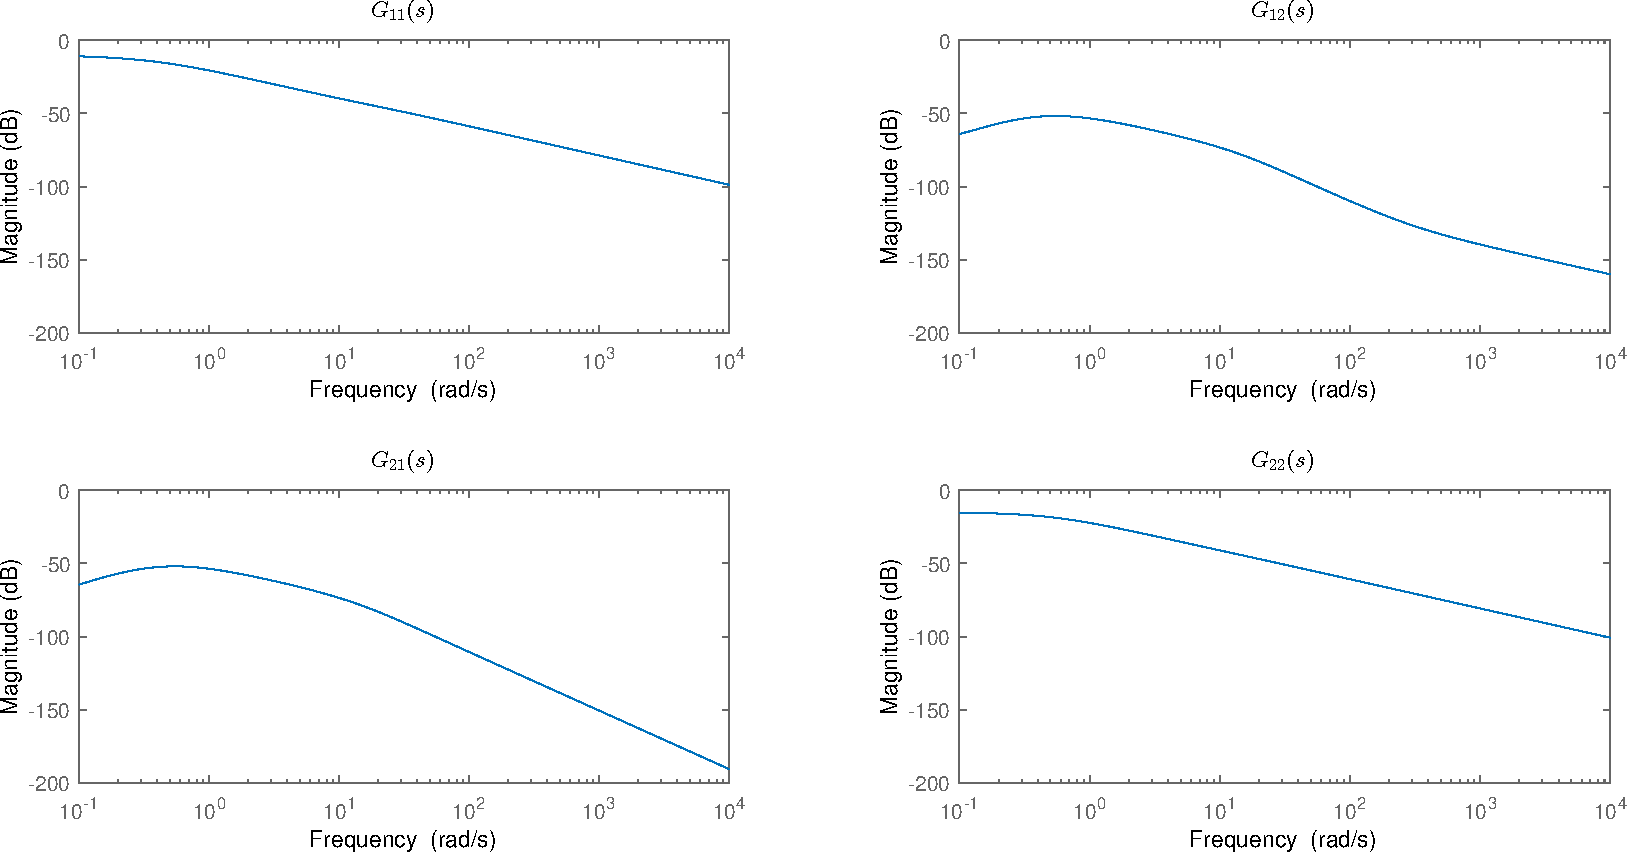
\includegraphics[width=\linewidth,height=4cm]{Graphics/BodeMagDelayPlot.pdf}
 	\caption{Transfer matrix magnitude plots, output delay included}
 	\label{fig:BodeMagDelayPlot}
\end{figure}

\newpage

On account of this the PID controllers for pump speeds $\omega_1$ and $\omega_2$ can be designed as SISO controllers without decoupling. Their poles and zeros are respectively:

\begin{equation}\label{eq:PumpTFNumDen}
	\begin{gathered}
		z_{11} = \begin{bmatrix}-18.92 & -14.00 & -0.56 & -0.34 & -0.19	\end{bmatrix} \\
		z_{22} = \begin{bmatrix}-20.72 & -14.10 & -0.41 & -0.36 & -0.16	\end{bmatrix} \\
		p_{11} = \begin{bmatrix}-20.77 & -14.86 & -0.56 & -0.39 & -0.33 & -0.16\end{bmatrix} \\
		p_{22} = \begin{bmatrix}-20.77 & -14.86 & -0.56 & -0.39 & -0.33 & -0.16\end{bmatrix}
	\end{gathered}
\end{equation}

Clearly many of these poles and zeros are approximately cancelling, and \cref{fig:BodeMagDelayPlot} indicates that $G_{11}(s) \approx G_{22}(s)$, so \cref{eq:PumpTFNumDen} can, for design purposes, be simplified to:

\begin{equation}\label{eq:PumpTFSimple}
	\begin{gathered}
		z_{11} = z_{22} = \begin{bmatrix}-0.19\end{bmatrix} \\
		p_{11} = p_{22} = \begin{bmatrix}-0.39 & -0.16 \end{bmatrix}
	\end{gathered}
\end{equation}

A PI controller is designed (i.e., the D term is $0$) via the root-locus method \cite{Franklin}, with the goal of no overshoot to avoid ringing and accompanying pressure oscillations in the pipes. To accommodate the presence of an outer loop and allow this to operate at a reasonable sample rate, a bandwidth of $0.05 \frac{\si{rad}}{\si{s}}$ is chosen. Note that per \cite{Skogestad2005}, a stable controller cannot be designed with a closed-loop bandwidth higher than $\frac{1}{T_{delay}} = 0.25 \frac{\si{rad}}{\si{s}}$. The resulting controller is:

\begin{equation}\label{eq:PIDTransferFunction}
	C(s) = 1.8\frac{s+0.05}{s}
\end{equation}


%\begin{equation}\label{eq:InfLQRHamiltonian}
%	\mathcal{H}(x(t),u(t),\lambda(t),t)) = \lambda^T(t)\big(Ax(t) + Bu(t)\big) - x^T(t)Qx(t) - u^T(t)Ru(t)
%\end{equation}





